\documentclass[border=10pt]{standalone}
\usepackage[svgnames]{xcolor}
\usepackage{amsmath}
\usepackage{pgfplots}
\pgfplotsset{compat=newest}
\usepackage[sfdefault]{FiraSans}
\usepackage{FiraMono}
\renewcommand*\familydefault{\sfdefault}
\begin{document}
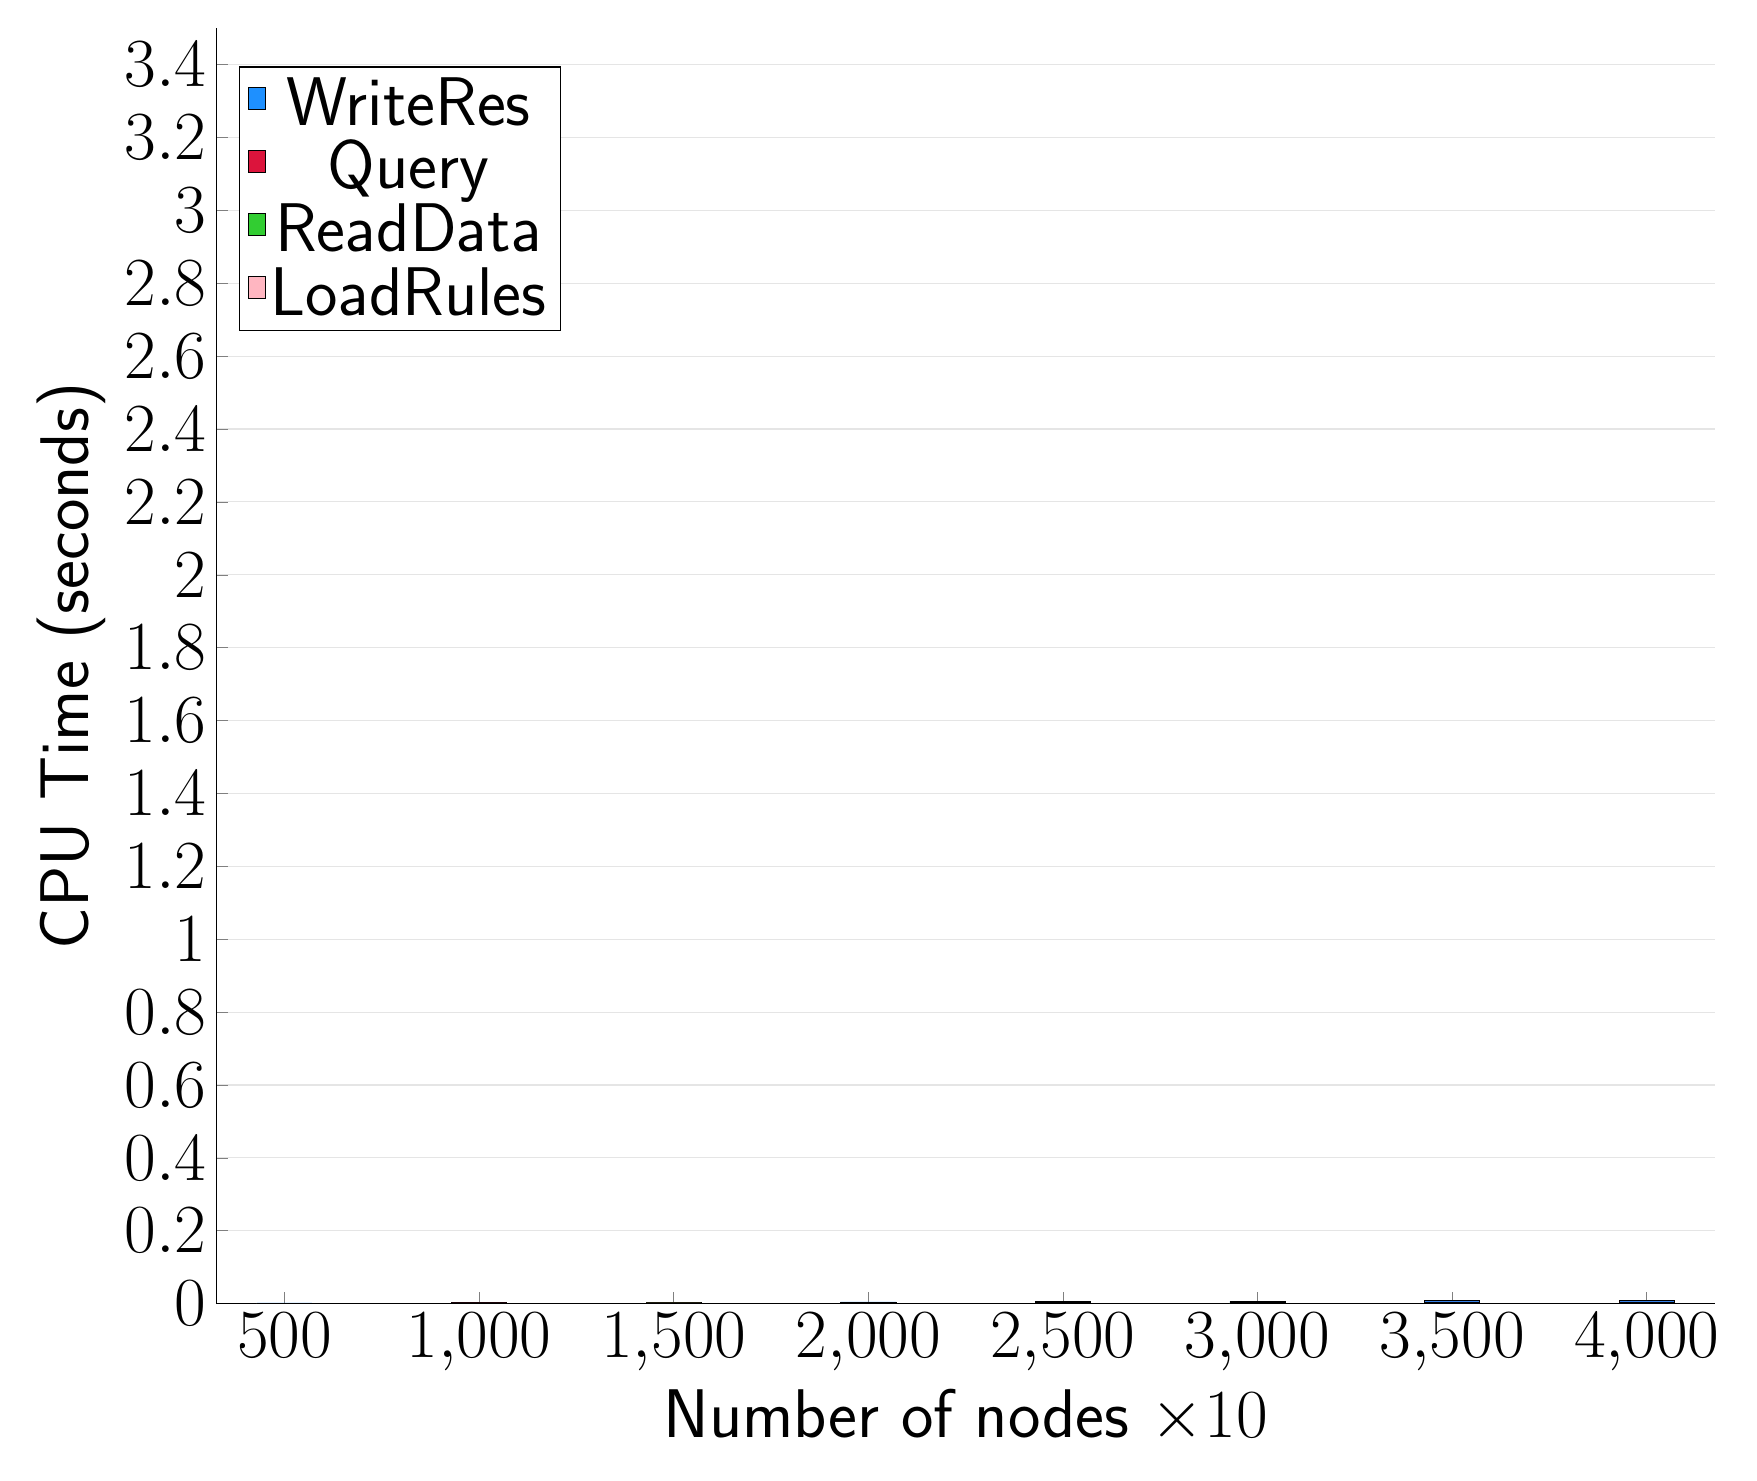
\begin{tikzpicture}
\begin{axis}[
   ybar stacked,
   width=1.7\textwidth,
   bar width=0.7cm,
   ymajorgrids, tick align=inside,
   major grid style={draw=gray!20},
   xtick=data,
   ymin=0, ymax=3.5,
   axis x line*=bottom,
   axis y line*=left,
   enlarge x limits=0.05,
   legend style={
       at={(0.23, 0.97)},
       anchor=north east,
       legend columns=1,
       font=\Huge,
   },
   ylabel={CPU Time (seconds)},
   xlabel={Number of nodes $\times 10$},
   label style={font=\Huge},
   tick label style={font=\Huge},
]
\addlegendimage{fill=DodgerBlue, draw=black, line width=0.2pt}
\addlegendentry{WriteRes}
\addlegendimage{fill=Crimson, draw=black, line width=0.2pt}
\addlegendentry{Query}
\addlegendimage{fill=LimeGreen, draw=black, line width=0.2pt}
\addlegendentry{ReadData}
\addlegendimage{fill=LightPink, draw=black, line width=0.2pt}
\addlegendentry{LoadRules}
\addplot +[fill=LightPink, draw=black, line width=0.2pt] coordinates {
(500, 0.0006322000000000002)
(1000, 0.0005981000000000004)
(1500, 0.0006065999999999999)
(2000, 0.0006004000000000002)
(2500, 0.0006501)
(3000, 0.0006298999999999999)
(3500, 0.0006483000000000002)
(4000, 0.0006143999999999996)
};
\addplot +[fill=LimeGreen, draw=black, line width=0.2pt] coordinates {
(500, 0.0005545000000000002)
(1000, 0.0009797)
(1500, 0.0014429)
(2000, 0.0018847000000000002)
(2500, 0.0023991000000000004)
(3000, 0.0027885999999999996)
(3500, 0.0032934000000000006)
(4000, 0.0036812)
};
\addplot +[fill=Crimson, draw=black, line width=0.2pt] coordinates {
(500, 7.79e-05)
(1000, 0.0001415999999999998)
(1500, 0.0002112999999999995)
(2000, 0.0002722000000000004)
(2500, 0.00034920000000000025)
(3000, 0.0004187999999999997)
(3500, 0.0005028000000000001)
(4000, 0.0005529000000000005)
};
\addplot +[fill=DodgerBlue, draw=black, line width=0.2pt] coordinates {
(500, 0.0005295000000000003)
(1000, 0.0009634000000000002)
(1500, 0.0014229000000000004)
(2000, 0.0018836999999999999)
(2500, 0.0024296)
(3000, 0.0029121)
(3500, 0.0034002)
(4000, 0.003871899999999999)
};
\end{axis}
\end{tikzpicture}

\end{document}
